\documentclass[
  aspectratio=169,
]{beamer}
\usepackage{algorithm}
\usepackage{algorithmic}
\usepackage[spanish]{babel}
\usepackage[utf8]{inputenc}
\usepackage[T1]{fontenc}
\usepackage{booktabs}
\usepackage{amsmath}
\usepackage{mathtools}
\usepackage{subfigure}
\usepackage{hyperref}
\usepackage{xcolor}
\usetheme[
  workplace=teiresias,
]{MU}

\graphicspath{{./imagenes/ResultadosNumericos/RightAngeCantilever/},{./imagenes/ResultadosNumericos/CantieleverPendulum/},{./imagenes/ResultadosNumericos/SimpleCable/},{./imagenes/ResultadosNumericos/TransmissionTormenta/}, {./imagenes/Preliminares/Corrotacional/},{./imagenes/Preliminares/deslizamientoRelativo/},{./imagenes/ResultadosNumericos/uniformCantilever/},{./imagenes/Metodologia/},{/imagenes/Anexo/}{./imagenes/Introduccion/}}


%%%%%%%%%%%%%%%%%%%%%%%%%%%%%%%%%%%%%%%%%%% BEGIN DOCUMENT %%%%%%%%%%%%%%%%%%%%%%%%%%%%%%%%%%%%%
 \begin{document}
	\begin{small}

\title[Programa de posgrado]{Titulo del trabajo  }
\subtitle[Curso]{Subtitulo del trabajo}
\author[Autor abrev.]{
	Autor1: Nombre$^\text{affiliación}$  
	\\Autor2: Nombre$^\text{affiliación}$   
	\\Autor3: Nombre$^\text{affiliación}$  
 }
\institute [IIMPI-IET]{1-Instituto de Ingeniería Mecánica y Producción Industrial, Facultad de Ingeniería, UdelaR \\ 2-Instituto de Estructuras y Transporte, Facultad de Ingeniería UdelaR  }
\date{\today}
\keywords{Palabra clave 1, Palabra clave 2, Palabra clave 3. }

%%%%%%%%%%%%%%%%%%%%%%%%%%%%%%%%%%    FRAME   %%%%%%%%%%%%%%%%%%%%%%%%%%%%%%%%%%%
\begin{frame}[plain]
	\maketitle
\end{frame}
%%%%%%%%%%%%%%%%%%%%%%%%%%%%%%%%%%    FRAME   %%%%%%%%%%%%%%%%%%%%%%%%%%%%%%%%%%%
\begin{frame}{Tabla de contenidos:}
	\tableofcontents
\end{frame}
%%%%%%%%%%%%%%%%%%%%%%%%%%%%%%%%%%%%%%%%     SECTION  %%%%%%%%%%%%%%%%%%%%%%%%%%%%%%%%%%%%%%%%%
\section[Introducción y preliminares]{Introducción y preliminares}
\AtBeginSection[]
{
	\begin{frame}
		\frametitle{Metodología}
		\tableofcontents[currentsection]
	\end{frame}
}
%%%%%%%%%%%%%%%%%%%%%%%%%%%%%%%%%%    SUBSECTION   %%%%%%%%%%%%%%%%%%%%%%%%%%%%%%%%%%%
\subsection[Agradecimientos]{Agradecimientos}
\begin{frame}{Agradecimientos:}{}
	\begin{block}{Gracias a:}
	\begin{itemize}
%		\pause
		\item Agradecimiento 1.
		\pause
		\item Agradecimiento 2.
		\pause
		\item Agradecimiento 3.  
	\end{itemize}
	\end{block}
\end{frame}
%%%%%%%%%%%%%%%%%%%%%%%%%%%%%%%%%%    SUBSECTION   %%%%%%%%%%%%%%%%%%%%%%%%%%%%%%%%%%%
\subsection[Introducción]{Introducción}
%%%%%%%%%%%%%%%%%%%%%%%%%%%%%%%%%%    FRAME   %%%%%%%%%%%%%%%%%%%%%%%%%%%%%%%%%%%
\begin{frame}
	\begin{block}{Motivación general:}
		\begin{itemize}
			\item Motivación general 1
			\pause
			\item Motivación general 2
			\pause
		\end{itemize}
	\end{block}
	\vfill
	\begin{block}{Motivación específica:}
		\begin{itemize}
			\item Motivación específica 1
			\pause
			\item Motivación específica 2
		\end{itemize}
	\end{block}
\end{frame}

%%%%%%%%%%%%%%%%%%%%%%%%%%%%%%%%%%    FRAME   %%%%%%%%%%%%%%%%%%%%%%%%%%%%%%%%%%%
\begin{frame}{Presentación del problema:}{}
	Ejemplo de imágen utilizando subfigure: 
	\begin{figure}[htbp]
		\centering
		\subfigure[Caption 1 ]{	\def\svgwidth{35mm}
			\input{./imagenes/Introduccion/Torre.pdf_tex}}
		\subfigure[Caption 2 con link a \href{https://www.clarin.com/sociedad/fenomeno-galloping-cayeron-torres-alta-tension-patagonia_0_fc3FYz1O-.html}{\structure{Noticia Clarín}}]{\includegraphics[width=0.45\textwidth]{./imagenes/Introduccion/TorreColapsada.jpg}}
	\end{figure}
\end{frame}

%%%%%%%%%%%%%%%%%%%%%%%%%%%%%%%%%%    FRAME   %%%%%%%%%%%%%%%%%%%%%%%%%%%%%%%%%%%
\begin{frame}{Ejemplo figura simple:}{}
	Ejemplo de imágen utilizando figure: 
	\begin{figure}[htbp]
		\centering
		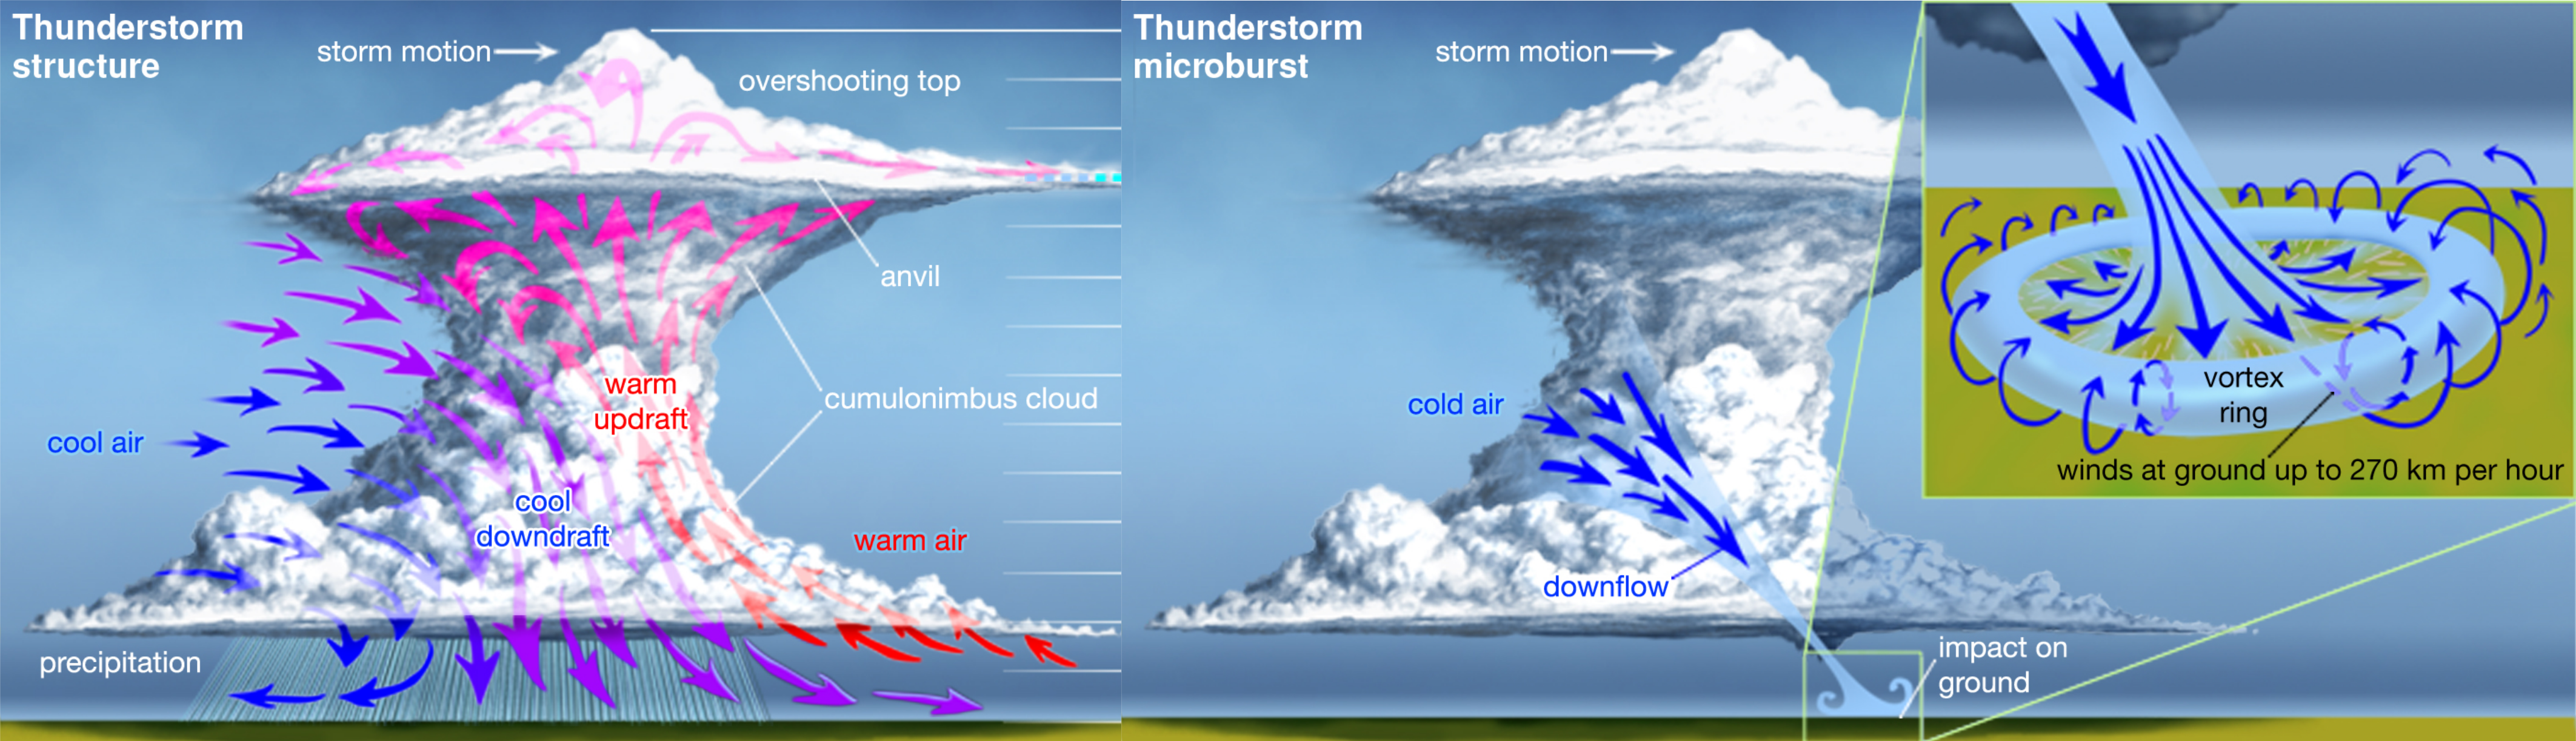
\includegraphics[width=1\textwidth]{./imagenes/Introduccion/ilusTormentasConvectivas.png}
		\caption{ Ejemplo con link de referencia \href{https://www.britannica.com/science/thunderstorm}{\structure{Encyclopedia britannica}}}
	\end{figure}
\end{frame}
% Agregar las causas


%%%%%%%%%%%%%%%%%%%%%%%%%%%%%%%%%%    FRAME   %%%%%%%%%%%%%%%%%%%%%%%%%%%%%%%%%%%
\begin{frame}{Ejemplos de box:}{}

\begin{alertblock}{¡Cambio climático!}
	Según {\color{blue}(Autor,año)} bla bla.
\end{alertblock}

\pause

\begin{block}{¿Cómo?}
	\begin{itemize}
		\item Ítem 1.
		\item Ítem 2.
		\item Ítem 3.
	\end{itemize}
\end{block}	


\end{frame}


%%%%%%%%%%%%%%%%%%%%%%%%%%%%%%%%%%%%%%%%FRAME%%%%%%%%%%%%%%%%%%%%%%%%%%%%%%%%%%%%%%%%%
\begin{frame}{Ejemplos de ecuaciones:}{}

	\begin{block}{Ecuación 1:}
		\begin{equation}\label{Eq:MET:EquilibrioExacto}
				\bf{f}_{ext,t+\delta_t}-\bf{f}_{int,t+\delta_t}-\bf{f}_{ine,t+\delta_t}=0
		\end{equation}
	\end{block}
\vfill
\begin{block}{Ecuación 2:}
	\begin{equation}\label{Eq:MET:Resto}
		\begin{split}
			\bf{r}(\bf{d}_{t+\delta_t})&=(-\bf{f}_{ext,t+\delta_t}+\bf{f}_{int}(\bf{d}_{t+\delta_t})+...\\	
			&...+\bf{f}_{ine}(\bf{d_{t+\delta_t}},\bf{v}_{t+\delta_t}(d_{t+\delta_t},\bf{d_t},\bf{v_t},\bf{a_t}),
			\bf{a}_{t+\delta_t}(d_{t+\delta_t},\bf{d_t},\bf{v_t},\bf{a_t}))
			\approx 0
		\end{split}
		\end{equation}
		\begin{equation}\label{Eq:MET:Residuo}
		\bf{r}(\bf{d}^{k+1}_{t+\delta_t})=\bf{r}(\bf{d}^k_{t+\delta_t}) +
		\frac{\partial  \bf{r}(\bf{d}_{t+\delta_t})}{\partial
			\bf{d}_{t+\delta_t}}|_k~\delta \bf{d}^{k+1}_{t+\delta_t}=0.
	\end{equation}
\end{block}
\end{frame}

%%%%%%%%%%%%%%%%%%%%%%%%%%%%%%%%%%%%%%%%%%%%%%%%FRAM%%%%%%%%%%%%%%%%%%%%%%%%%%%%%
\begin{frame}{Ejemplo sub-pagina.}
	\begin{minipage}[t]{0.4\linewidth}
		\begin{block}{Box de texto:}
			\begin{itemize}
				\item Ítem 1.
				\item Ítem 2. 
				\item Ítem 3.
			\end{itemize}
		\end{block}
	\end{minipage}
	\hspace{1cm}
	\begin{minipage}[t]{0.5\linewidth}
		\vspace{-1.8cm}
		\begin{block}{Ecuación 1:}
			\begin{equation}
			\begin{split}
			\bf{r}^{\text{$HHT$}}&=(1+\alpha_\text{$HHT$})(-\bf{f}_{ext,t+\delta_t}+\bf{f}_{int,t+\delta_t}+\bf{f}_{vis,t+\delta_t})...\\
			&...-\alpha_\text{$HHT$}(-\bf{f}_{ext,t}+\bf{f}_{int,t}+\bf{f}_{vis,t})+...\\
			&...+\bf{f}_{ine,t+\delta_t}	\approx 0
			\end{split}
			\end{equation}
		\end{block}
		\begin{block}{Ecuación 2:}
			\begin{equation}\label{Eq:MET:FinalIncremento}
			\begin{split}
			\bf{K}_{tot}= (1+\alpha_{HHT})&\bf{K}_g+{\left( \frac{4}{(1-\alpha_{HHT}^2) \delta_t^2} \right)} \bf{M}\bf{B}_t...\\ &...\left({\frac{1^2+\alpha^2_{HHT}}{2\delta_t}}\right) (\bf{C}_k+\bf{C}_{vis}) \bf{B}_t 
			\end{split}
			\end{equation}
		\end{block}
	\end{minipage}
\end{frame}


%%%%%%%%%%%%%%%%%%%%%%%%%%%%%%%%%%%%%%%%FRAME%%%%%%%%%%%%%%%%%%%%%%%%%%%%%%%%%%%%%%%%%

\begin{frame}{Ejemplo con subpage-tablas y figuras:}{}
	\begin{minipage}[t]{0.5\linewidth}
		\begin{figure}[htbp]
			\centering
			\def\svgwidth{60mm}
			\input{./imagenes/Preliminares/Corrotacional/IlusCorrotacional2.pdf_tex}
		\end{figure}
	\end{minipage}\hfill
	\begin{minipage}[t]{0.5\linewidth}
		\begin{table}[htbp]
			\begin{tabular}{|c|c|}
				\hline
				Matriz & Vínculo de sistemas de referencia \\
				\hline \hline
				$\bf{R}_0$ &$(\bf{E_1},\bf{E_2},\bf{E_3})$ $\rightarrow$
				$(\bf{e_1},\bf{e_2},\bf{e_3})$   \\ \hline
				$\bf{R}_i^g$ & $(\bf{e_1},\bf{e_2},\bf{e_3})$ $\rightarrow$
				$(\bf{t_1^i},\bf{t_2^i},\bf{t_3^i})$ \\ \hline
				$\bf{\overline{R}}_i$ &
				$(\bf{r_1},\bf{r_2},\bf{r_3})$$\rightarrow$$(\bf{t_1^i},\bf{t_2^i},\bf{t_3^i})$
				\\ \hline
				$\bf{R}_r$ &
				$(\bf{t_1^i},\bf{t_2^i},\bf{t_3^i})$$\rightarrow$$(\bf{r_1},\bf{r_2},\bf{r_3})$ \\
				\hline
			\end{tabular}
			%		\caption{Caracterización de matrices en términos de los sistemas de referencia.}
		\end{table}
		\begin{block}{¿Como calcular $\bf{\overline{R}}_i$? }
			\begin{eqnarray}
			\bf{R_i^g}\bf{R_o}&=& \bf{R_r}\overline{\bf{R_i}}\\
			\bar{\bf{R_i}}&=&(\bf{R_r})^T\bf{R_i^g}\bf{R_o}
			\end{eqnarray}
		\end{block}
	\end{minipage}	
\end{frame}



%%%%%%%%%%%%%%%%%%%%%%%%%%%%%%%%%%%%%%%     SECTION  %%%%%%%%%%%%%%%%%%%%%%%%%%%%%%%%%%%%%%%%%
\section[Metodología]{Metodología}

\AtBeginSection[]
{
	\ifnum \value{framenumber}>1
	\begin{frame}<beamer>
		\frametitle{Resultados}
		\tableofcontents[currentsection]
	\end{frame}
	\else
	\fi
}
%%%%%%%%%%%%%%%%%%SUBSECTION%%%%%%%%%%%%%%%%%%
\subsection[Subsección Metodología 1 ]{Subsección Metodología 1}

%%%%%%%%%%%%%%%%%%%%%%%%%%%%%%%%%%%%%%%%FRAME%%%%%%%%%%%%%%%%%%%%%%%%%%%%%%%%%%%%%%%%%
\begin{frame}{Ejemplo figura y box de texto:}
		\begin{minipage}[t]{0.35\linewidth}
		\begin{figure}[htbp]
			\centering
			\def\svgwidth{50mm}
			\input{./imagenes/Metodologia/EsquemaInicial.pdf_tex}
%				\caption{Esquema del objeto de estudio.}
		\end{figure}
		\end{minipage}\hfill
		\begin{minipage}[t]{0.64\linewidth}
			\begin{block}{Block de texto:}
				\begin{itemize}
				\item Ítem 1.
				\pause
				\item Ítem 2.
				\pause
				\item Ítem 3.
				\end{itemize}
			\end{block}
		\end{minipage}
\end{frame}
%%%%%%%%%%%%%%%%%%%SUBSECTION%%%%%%%%%%%%%%%%%%

\subsection[Subsección Metodología 2 ]{Subsección Metodología 2}

%%%%%%%%%%%%%%%%%%%%%%%%%%%%%%%%%%%%%%%%%%%FRAME%%%%%%%%%%%%%%%%%%%%%%%%%%%%%%%%%%%%%%%%%
%%%%%%%%%%%%%%%%%%%%%%%%%%%%%%%%%%%%%%%%%     SECTION  %%%%%%%%%%%%%%%%%%%%%%%%%%%%%%%%%%%%%%%%%
 \section[Resultados Numéricos]{Resultados Numéricos}
\subsection[Resultado 1 Abv]{Resultado 1}
%%%%%%%%%%%%%%%%%%%%%%%%%%%%%%%%%%%%%%%%%%FRAME%%%%%%%%%%%%%%%%%%%%%%%%%%%%%%%%%%%%%%%%%
\begin{frame}[t]{Ejemplo de sub-column y sub-page:}
	\begin{columns}[T,onlytextwidth]
		\begin{column}{.58\textwidth}
			\begin{minipage}{\textwidth}
				\begin{figure}[htbp]
				\subfigure[Vista frontal ]{	\def\svgwidth{30mm}
				\input{./imagenes/ResultadosNumericos/RightAngeCantilever/Ilustracion2Dxy.pdf_tex}}\label{fig:RN:RA:Ilusxy}
				\subfigure[Vista lateral ]{	\def\svgwidth{20mm}
				\input{./imagenes/ResultadosNumericos/RightAngeCantilever/Ilustracion2Dyz.pdf_tex}}\label{fig:RN:RA:Ilusyz}
%				\caption{Disposición geométrica de la estructura.} 	\label{fig:RN:RA:esquemas}
				\end{figure}
					\begin{figure}[htbp]
					
					\def\svgwidth{35mm}
					\input{./imagenes/ResultadosNumericos/RightAngeCantilever/FuerzaZ.pdf_tex}
%					\caption{Perfil de fuerza $F_z$}
				\end{figure}
		\end{minipage}  
		\end{column}
		\begin{column}{.4\textwidth}
			\begin{onlyenv}<2->
				\begin{minipage}{\textwidth}
					\vspace{-1cm}
					\begin{block}{Box 1:}
						\begin{itemize}
							\item Ecuaciones: $GA= EA=10^6$ y $GJ = EI =10^3$.  

						\end{itemize}	 
					\end{block}
				\end{minipage}
			\end{onlyenv}
			\begin{onlyenv}<3->
				\begin{minipage}{\textwidth}
					\begin{block}{Box 2:}
						\begin{itemize}
							\item Texto.
						\end{itemize}	 
					\end{block}
				\end{minipage}
			\end{onlyenv}
		\end{column}
	\end{columns}
\end{frame}
%%%%%%%%%%%%%%%%%%%%%%%%%%%%%%%%%%%%%%%%     SECTION  %%%%%%%%%%%%%%%%%%%%%%%%%%%%%%%%%%%%%%%%%
\section[Conclusiones]{Conclusiones}

\AtBeginSection[]
{
	\ifnum \value{framenumber}>1
	\begin{frame}<beamer>
		\frametitle{}
		\tableofcontents[currentsection]
	\end{frame}
	\else
	\fi
}
%%%%%%%%%%%%%%%%%%%%%%%%%%%%%%%%%%%%%%%%%%FRAME%%%%%%%%%%%%%%%%%%%%%%%%%%%%%%%%%%%%%%%%%
\begin{frame}{Conclusiones }
	\begin{itemize}
		\item  Conclusión 1. 
		\pause 
		\item  Conclusión 2. 
		\pause
		\item  Conclusión 3. 
	\end{itemize}
\end{frame}
%%%%%%%%%%%%%%%%%%%%%%%%%%%%%%%%%%%%%%%%%%FRAME%%%%%%%%%%%%%%%%%%%%%%%%%%%%%%%%%%%%%%%%%
\begin{frame}{Trabajos a futuro }
	\begin{itemize}
		\item Trabajo 1.
		\pause
		\item Trabajo 2.
		\pause
		\item Trabajo 3.
	\end{itemize}
\end{frame}

%%%%%%%%%%%%%%%%%%%%%%%%%%%%%%%%%%%%%%%%%%FRAME%%%%%%%%%%%%%%%%%%%%%%%%%%%%%%%%%%%%%%%%%
\begin{frame}[t]{Gracias:}
	\begin{alertblock}{Gracias...}
		¡!
	\end{alertblock}
\pause
\begin{alertblock}{¿Preguntas?}
	¿? 
\end{alertblock}
\end{frame}
%%%%%%%%%%%%%%%%%%%%%%%%%%%%%%%%%%%%%%%%%%FRAME%%%%%%%%%%%%%%%%%%%%%%%%%%%%%%%%%%%%%%%%%
\begin{frame}{Referencias principales:}
	\begin{itemize}
		\item {\color{blue}(Le,2014)}: Le, T. N., Battini, J. M. y Hjiaj, M. (2014). A consistent 3D corotational beam element for nonlinear dynamic analysis of exible structures. Computer Methods in Applied Mechanics and Engineering, 269, 538-565.
		\item {\color{blue}(Viera,1969)} : Vieira, S.E., 1969. Tiempo y Clima, ed. nuestra tierra, vol. 8, 68pp.
		\item {\color{blue}(Li,2000)}: Li, C.Q., 2000. A stochastic model of severe thunderstorms for transmission line design. Probabilist. Eng. Mech. 15 (4), 359–364.
		\item{\color{blue}(Crisfield,1997)} Crisfield, M. A. (1997). Non-linear finite element analysis of solids and structures, Vol. 2. John Wiley and Sons.
		\item{\color{blue}(Simo y  Vu-Quoc ,1988) }Simo, J. C. y Vu-Quoc, L. (1988). On the dynamics in space of rods undergoing large motions and geometrically exact approach. Computer methods in applied mechanics and engineering, 66 (2), 125-161.
	\end{itemize}
\end{frame}

%%%%%%%%%%%%%%%%%%%%%%%%%%%%%%%%%%%%%%%%%FRAME%%%%%%%%%%%%%%%%%%%%%%%%%%%%%%%%%%%%%%%%%

\begin{frame}{Referencias principales:}
	\begin{itemize}
		\item {\color{blue}(Durañona,2019)}: Durañona, V., Marchesoni, E. y Salles, R. (2019). A first characterization of high winds that afect the energy distribution system of Uruguay and their related facts. Journal of Wind Engineering and Industrial Aerodynamics, 128-138.
		\item{\color{blue}(Stengel,2017)} Stengel, D. y Thiele, K. (2017). Measurements of downburst wind loading acting on an overhead transmission line in Northern Germany. Procedia engineering, 199, 3152-3157.
 		\item {\color{blue}(Foti,2016)} Foti, F. y Martinelli, L. (2016). An analytical approach to model the hysteretic bending behavior of spiral strands. Applied Mathematical Modelling, 40 (13-14), 6451-6467. https://doi.org/10.1016/j.apm.2016.01.06318 001
 		\item {\color{blue}(Foti,2018)} Foti, F. y Martinelli, L. (2018). Finite element modeling of cable galloping vibrations. Part II: Application to an iced cable in 1: 2 multiple internal resonance. Journal of Vibration and Control, 24 (7), 1322-1340.
	\end{itemize}
\end{frame}


%%%%%%%End document
	\end{small}
\end{document}
